\documentclass[14pt, a4paper]{article}
\usepackage{fullpage}
\usepackage[top=2cm, bottom=2cm, left=2.5cm, right=2cm]{geometry}
\usepackage{amsmath,amsthm,amsfonts,amssymb,amscd}
\usepackage{fancyhdr}
\usepackage{fixltx2e}
\usepackage{mathrsfs}
\usepackage{listings}
\usepackage{color}
\usepackage{relsize}
\usepackage{graphicx}
\usepackage[utf8]{inputenc}
\usepackage[T1]{fontenc}
\usepackage[english, russian]{babel}

\definecolor{dkgreen}{rgb}{0,0.6,0}
\definecolor{gray}{rgb}{0.5,0.5,0.5}
\definecolor{mauve}{rgb}{0.58,0,0.82}

\DeclareMathSizes{14}{24}{18}{12}

\lstset{frame=tb,
  language=Python,
  aboveskip=3mm,
  belowskip=3mm,
  showstringspaces=false,
  columns=flexible,
  basicstyle={\small\ttfamily},
  numbers=none,
  numberstyle=\tiny\color{gray},
  keywordstyle=\color{blue},
  commentstyle=\color{dkgreen},
  stringstyle=\color{mauve},
  breaklines=true,
  breakatwhitespace=true,
  tabsize=3
}

\renewcommand{\thesection}{\arabic{section}.}
\renewcommand{\thesubsection}{\thesection\arabic{subsection}.}
\renewcommand{\thesubsubsection}{\thesubsection\arabic{subsubsection}.}

\begin{document}
\pagenumbering{gobble}
\begin{titlepage}
\begin{center}
\large{БЕЛОРУССКИЙ ГОСУДАРСТВЕННЫЙ УНИВЕРСИТЕТ 

ФАКУЛЬТЕТ ПРИКЛАДНОЙ МАТЕМАТИКИ И ИНФОРМАТИКИ

КАФЕДРА ВЫЧИСЛИТЕЛЬНОЙ МАТЕМАТИКИ}
\end{center}
\vspace*{\fill}
\begin{center}
Лабораторная работа 11

\large{\textbf{Интерполирование функции с использованием сетки равноотстоящих узлов}}

Вариант 7
\end{center}
\begin{flushright}
\textbf{Выполнил:}

Журик Никита Сергеевич \\ 2 курс, 6 группа

\textbf{Преподаватель:}

Будник Анатолий Михайлович
\end{flushright}
\vspace*{\fill}
\begin{center}
Минск, 2019
\end{center}
\end{titlepage}

\tableofcontents
\newpage

\newpage
\pagenumbering{arabic}

  \section{Постановка задачи}
    \begin{enumerate}
      \item
      Интерполировать исходную функцию по равномерной системе узлов;
      \item
      Вычислить теоретическую оценку и действительную невязку интерполирования;
      \item
      Проанализировать результаты и сравнить с методом Ньютона.
    \end{enumerate}
  \section{Алгоритм решения}
  \begin{itemize}
     \item
     Рассмотрим задачу интерполирования исходной функции $f(x)$ в начале таблицы равноотстоящих узлов многочленом третьей степени.
     \item 
     Для интерполирования исходной функции воспользуемся аппаратом правых конечных разностей и формулой связи с разделёнными разностями: \begin{equation}f(x_0, \dots, x_k) = \frac{\Delta^kf_0}{k!h^k} \end{equation}
     Здесь $\Delta^kf_0$ - это ПКР $k$-го порядка, $h$ - расстояние между соседними узлами.
     \item
     Введём новую переменную: $t = \frac{x-x_0}{h}$. Тогда формула многочлена Ньютона может быть записана в следующем виде: \begin{equation}P_k(x) = P_k(x_0+th) = f_0 + \frac{t}{1!}\Delta f_0 + \frac{t(t-1)}{2!}\Delta^2f_0 + \dots + \frac{t(t-1)\dots(t-k+1)}{k!}\Delta^kf_0\end{equation}
     Воспользуемся этой формулой при $k=3$.
     \item
     С учётом приведённых выше рассуждений теоретическая оценка невязки будет иметь вид: \begin{equation}r_k(x) = r_k(x_0 + th) = h^{k+1}\frac{t(t-1)\dots(t-k)}{(k+1)!}f^{(k+1)}(\xi), \xi \in [x_0, x_0 + kh]\end{equation}
  \end{itemize}
  \section{Листинг программы}
  Для реализации алгоритма был использован Python и библиотеки numpy и matplotlib.

\begin{lstlisting}
#EquallySpaced.py

import numpy as np
from math import exp, log, factorial
import matplotlib.pyplot as plt

a = 1.0
b = 1.3
N = 3
delta = (b - a) / N
alpha = 1.7

points = [a + i * delta for i in range(N + 1)]

def f(x):
    return alpha * exp(-x) + (1 - alpha) * log(x)

def fDerivN1(x):
    return (-1) ** (N + 1) * alpha * exp(-x) + (1 - alpha) * ((-1) ** (N)) * factorial(N) / x ** (N + 1)

def maxDerivN1(samples):
    space = np.linspace(a, b, samples)
    return np.max(np.abs(np.array([(fDerivN1(x)) for x in space], dtype=np.double)))

def buildNewtonDiffs(points, f):
    A = np.zeros((N + 1, N + 2), dtype=np.double)
    for i in range(N + 1):
        A[i][0] = points[i]
        A[i][1] = f(points[i])
    for j in range(2, N + 2):
        for i in range(j - 1, N + 1):
            A[i][j] = (A[i][j - 1] - A[i - 1][j - 1]) / (A[i][0] - A[i - j + 1][0])
    return A

def buildDiffs(points, f):
    A = buildNewtonDiffs(points, f)
    return np.array([A[i][i + 1] * factorial(i) * delta ** i for i in range(N + 1)], dtype=np.double)

def prod(i):
    return lambda x: np.prod(np.array([(x - j) for j in range(i)], dtype=np.double))

def getSolution(diffs, points):
    return lambda x: np.sum(np.array([diffs[i] * prod(i)((x - points[0]) / delta) / factorial(i) for i in range(N + 1)],
                                     dtype=np.double))

def deficiency(x, diffs, points):
    t = (x - points[0]) / delta
    return abs(prod(N + 1)(t) * maxDerivN1(10000) * delta ** (N + 1) / factorial(N + 1))

def plotDifference(samples, solution):
    space = np.linspace(a, b, samples)
    plt.plot(space, np.zeros(np.shape(space)))
    plt.plot(space, np.array([solution(x) - f(x) for x in space], dtype=np.double))
    plt.savefig("../TeX/Interpolation/EquallySpacedDiff.png")
    plt.show()

if __name__ == "__main__":
    diffs = buildDiffs(points, f)
    solution = getSolution(diffs, points)
    
    check = [points[0] + delta / 2.6]
    
    [print("Pn({0}) = {1}".format(x, solution(x))) for x in check]
    print()
    
    [print("rn({0}) = {1}".format(x, solution(x) - f(x))) for x in check]
    print()
    
    print("Expected deficiency in control points: " + 
          str(np.max(np.abs(np.array([(deficiency(x, diffs, points)) for x in check], dtype=np.double)))))
    
    space = np.linspace(a, b, 1000)
    print("Real deficiency on whole interval: " + 
          str(np.max(np.abs(np.array([(solution(x) - f(x)) for x in space], dtype=np.double)))))
    print()
    
    print("Real deficiency in control points: " + 
          str(np.max(np.abs(np.array([(solution(x) - f(x)) for x in check], dtype=np.double)))))
    
    plotDifference(1000, solution)
\end{lstlisting}

  \section{Вывод программы}
\begin{verbatim}
Pn(1.0384615384615385) = 0.5753931462430032

rn(1.0384615384615385) = 1.328510657672144e-05

Expected deficiency in control points: 2.0105108747907392e-05
Real deficiency on whole interval: 1.329082616186028e-05

Real deficiency in control points: 1.328510657672144e-05
\end{verbatim}
\begin{figure}[h!]
  \center
  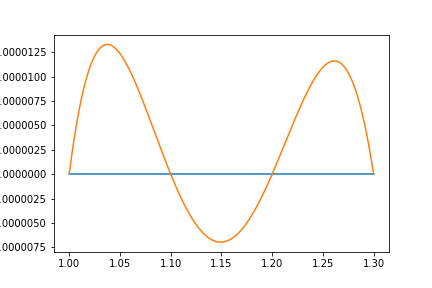
\includegraphics[width=0.6\linewidth]{EquallySpacedDiff.png}
  \caption{Невязка интерполирования}
\end{figure}

  \section{Выводы}
  \begin{itemize}
  \item
  В результате применения формул (1) и (2) удалось интерполировать исходную функцию многочленом третьей степени с точностью $r_{EqSp_{real}} = 1.329082616186028e-05$ (на всём отрезке $[1, 1.3]$), $r_{EqSp_{control}} = 1.328510657672144e-05$ (в рассматриваемой точке $x^*$), что удовлетворяет полученной оценке погрешности $r_{EqSp_{theor}} = 2.0105108747907392e-05$.
  \item
  Полученная при использовании рассмотренного метода точность высока для интерполяции многочленом третьей степени, однако он применим лишь к интерполяции в начале таблицы. Для расширения возможностей данного метода его реализацию следует дополнить формулами для интерполяции в середине и в конце таблицы.
  \end{itemize}

\end{document}